\documentclass{article}
\usepackage{amsmath}
\usepackage[margin=1in]{geometry}
\usepackage{graphicx}
\title{Bounded Visual Portrait Sculpting}
\date{2026-11-27}
\begin{document}
\maketitle
\section{Scope}
Issue 15847 extends the shared CC0 head for reference-directed portrait work.
These are artistic controls, not measured facial anthropometry. The original
five controls and their serialized form remain unchanged when the additions
are zero. Physical definitions, joints, collision geometry and inertia are
not inputs or outputs of this deformation.
\section{Coordinate Map}
Coordinates are head lengths: $x$ forward, $y$ left, $z$ up from the neck.
All signed controls lie in $[-0.2,0.2]$. New fields use the compact window
\[B(t;c,r)=\max(1-((t-c)/r)^2,0)^2.\]
It and its first derivative vanish at the boundary. Products of vertical and
lateral windows select cheeks, chin, brow, bridge, nose, eyelids and ears.
The source in \texttt{head\_morph.py} records each centre, radius and amplitude.
Bridge, brow and chin primarily change forward projection; cheek and chin
controls also change width. Nose width and length act independently. The eye
opening scales local vertical distance from $z=0.538$, and face length moves
lower-face vertices within a window centred at $z=0.39$ with radius $0.25$.
The top of the skull and neck plane therefore retain their original coordinates.
\section{Features and Invariants}
The same map deforms skin, eyes, facial hair and accessories. Brow prominence
also adjusts the shared eyebrow strip's thickness and slant before mapping.
Optional moustache strips use closed ellipsoids conformed to the original
upper-lip surface, then pass through the same deformation. They use the
existing darker hair material role and carry no physical mass or collision.
Tests cover public schema round trips, invalid input rejection, distinct
landmark effects, unchanged neck/skull extrema, closed facial-hair topology,
and exact native body/joint/dynamics equivalence at three states. Per-player
likeness needs inspection against attributed references; passing these tests
alone does not establish likeness. Body height retains the existing neutral
head-skin-to-lowest-shoe convention, excluding hair and headwear.
\section{Rendered Evidence}
The paired renders show a neutral portrait before and after one illustrative
sculpt. The changed view is not fitted to a historical photograph and is not a
player likeness claim. Desktop images are rendered at 1280 by 960 pixels and
phone images at 390 by 844 pixels with a separately fitted camera; neither is
resized before capture. Three-quarter and profile views are included with the paired front views.
\begin{figure}[ht]
\centering
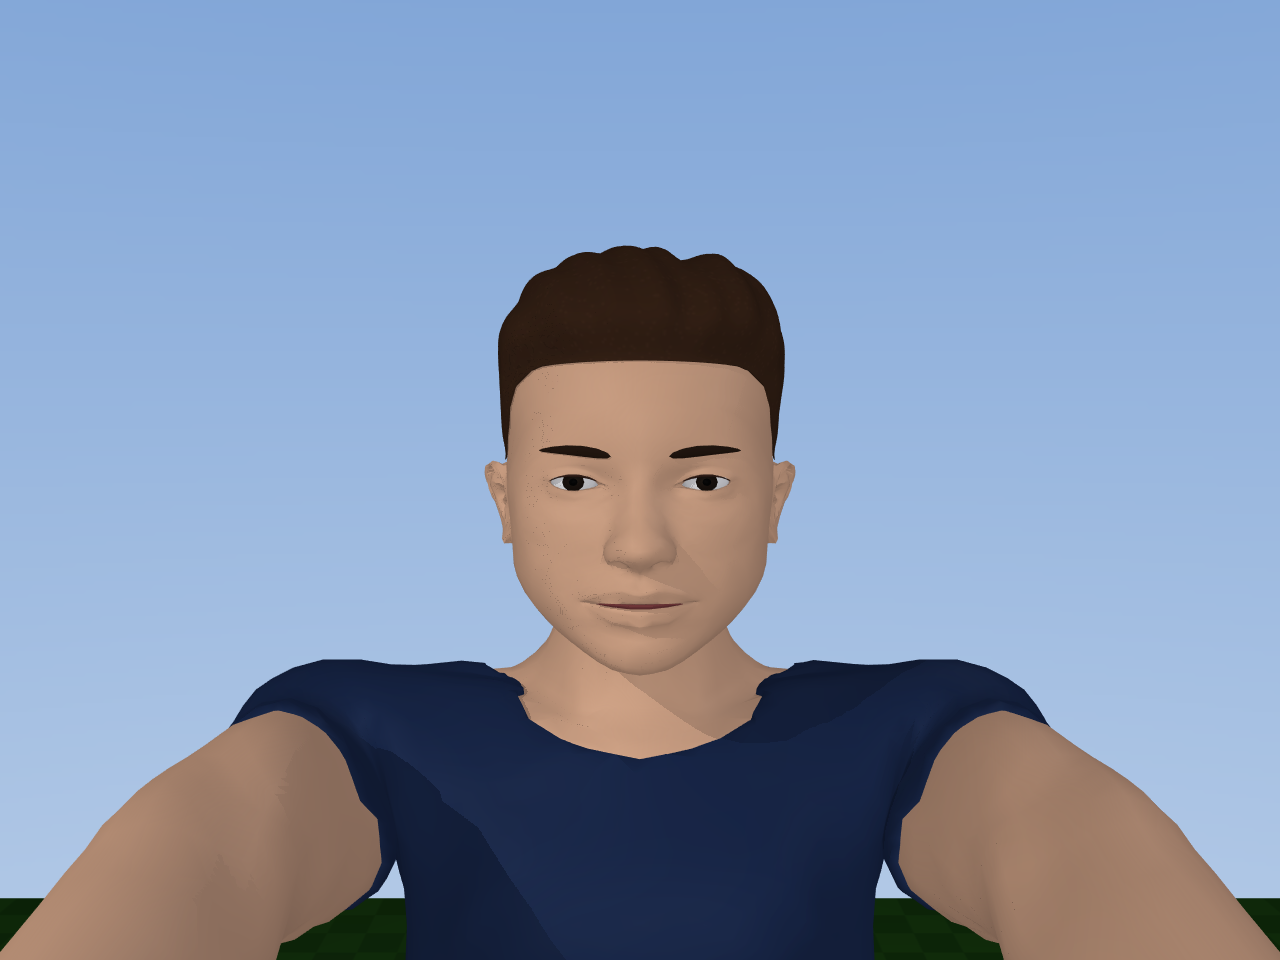
\includegraphics[width=0.47\linewidth]{docs/development/evidence/appearance/portrait_sculpt/before/front_1280x960.png}\hfill
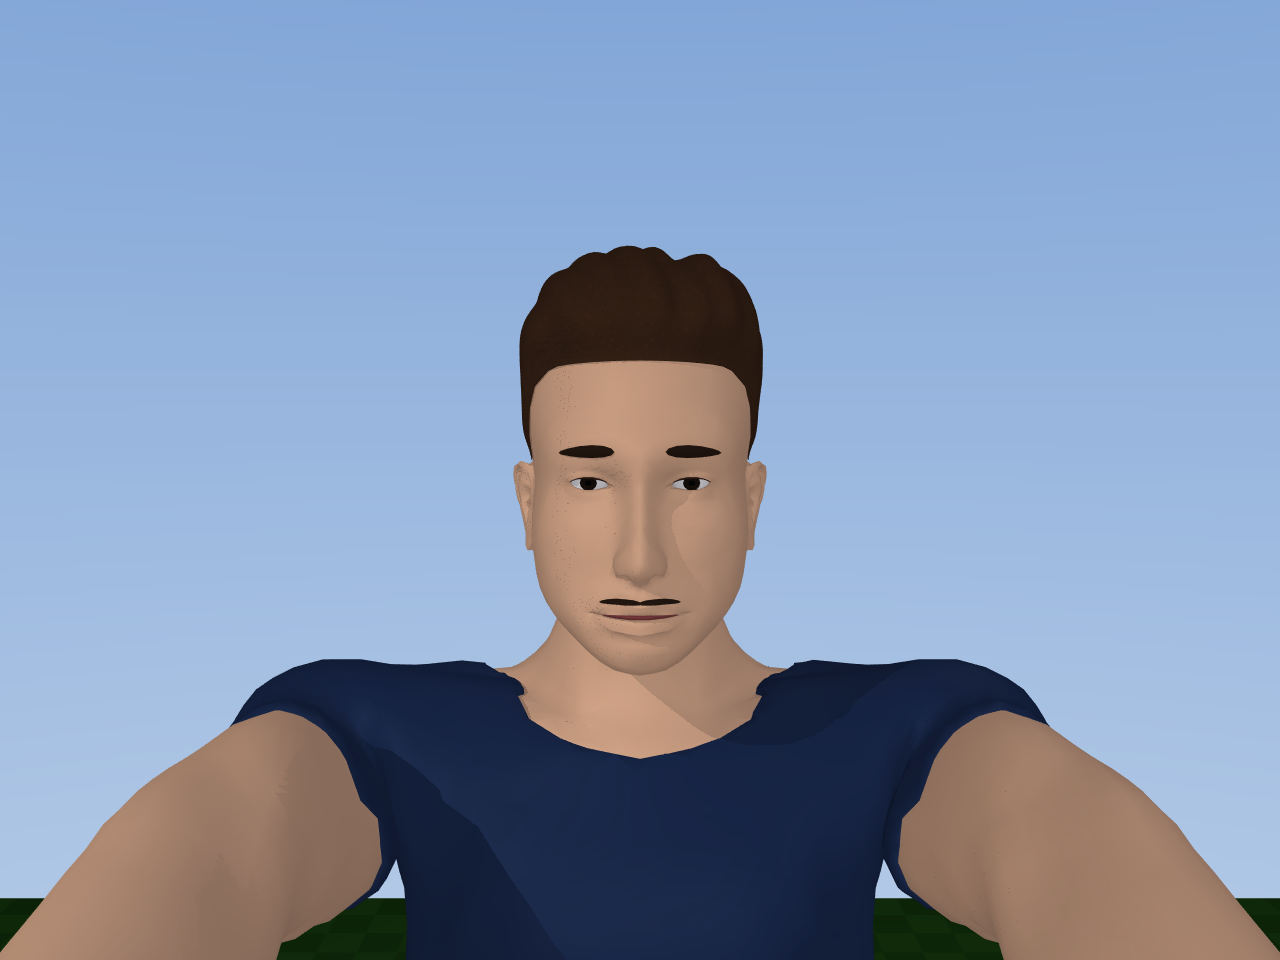
\includegraphics[width=0.47\linewidth]{docs/development/evidence/appearance/portrait_sculpt/after/front_1280x960.png}\\
Before (desktop)\hfill After (desktop)
\end{figure}
\begin{figure}[ht]
\centering
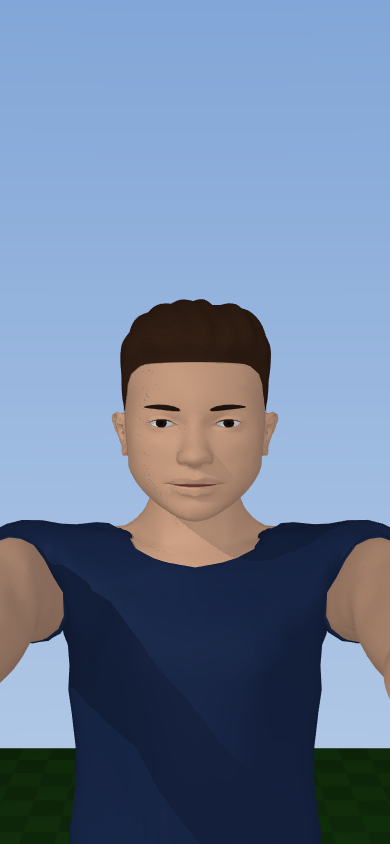
\includegraphics[width=0.24\linewidth]{docs/development/evidence/appearance/portrait_sculpt/before/front_390x844.png}\hfill
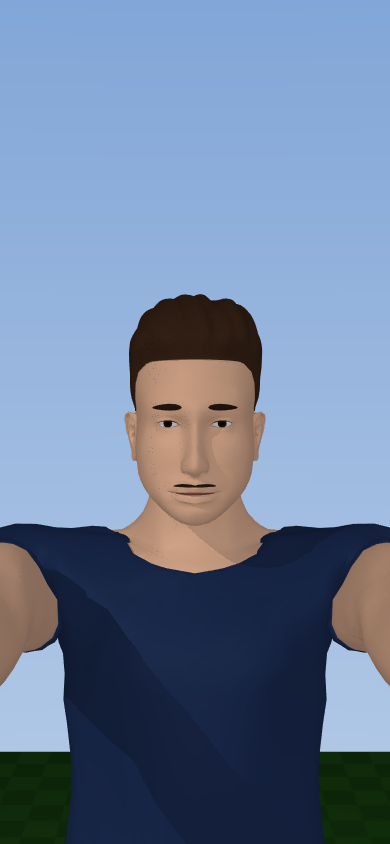
\includegraphics[width=0.24\linewidth]{docs/development/evidence/appearance/portrait_sculpt/after/front_390x844.png}\\
Before (phone)\hfill After (phone)
\end{figure}
The exact inputs and native renderer are reproducible from the evidence folder:
\begin{verbatim}
cd docs/development/evidence/appearance/portrait_sculpt
MUJOCO_GL=egl PYTHONPATH=../../../../..:../../../../../vendor/ud-tools/src \
  python3 render_portrait_sculpt.py --repo ../../../../.. --out .
\end{verbatim}
\end{document}
